\documentclass[aspectratio=169,10pt]{beamer}
\usepackage[utf8]{inputenc}
\usepackage[T1]{fontenc}
\usepackage[spanish]{babel}
\usepackage{lmodern}
\usepackage{graphicx}
\usepackage{booktabs}
\usepackage{tcolorbox}
\usepackage{array}

\definecolor{mxNavy}{HTML}{12405E}
\definecolor{mxBlue}{HTML}{2A85BE}
\definecolor{mxLight}{HTML}{EEF7FC}
\definecolor{mxGreen}{HTML}{206641}
\definecolor{mxWarn}{HTML}{B45309}

\usetheme{Madrid}
\usecolortheme{default}
\setbeamercolor{structure}{fg=mxNavy}
\setbeamercolor{palette primary}{bg=mxNavy,fg=white}
\setbeamercolor{palette secondary}{bg=mxBlue,fg=white}
\setbeamercolor{palette tertiary}{bg=mxNavy!85!black,fg=white}
\setbeamercolor{frametitle}{bg=mxNavy,fg=white}
\setbeamercolor{title}{bg=mxNavy,fg=white}
\setbeamercolor{block title}{bg=mxBlue,fg=white}
\setbeamercolor{block body}{bg=mxLight,fg=black}
\setbeamertemplate{navigation symbols}{}
\setbeamertemplate{footline}{
  \leavevmode\hbox{%
  \begin{beamercolorbox}[wd=.45\paperwidth,ht=2.4ex,dp=1ex,leftskip=1em]{palette primary}%
    \usebeamerfont{author in head/foot}ICN-292 · Grupo 2 · P100 · Maxilux
  \end{beamercolorbox}%
  \begin{beamercolorbox}[wd=.40\paperwidth,ht=2.4ex,dp=1ex,center]{palette secondary}%
    \usebeamerfont{title in head/foot}Entrega 2 — Solución SIG Final
  \end{beamercolorbox}%
  \begin{beamercolorbox}[wd=.15\paperwidth,ht=2.4ex,dp=1ex,rightskip=1em]{palette primary}%
    \hfill\insertframenumber{} / \inserttotalframenumber
  \end{beamercolorbox}}%
  \vskip0pt%
}

\title[Maxilux · Entrega 2]{Solución SIG Final para Maxilux}
\subtitle{De procesos manuales a automatización en n8n y base de datos 3FN auditable}
\author[Grupo 2 · P100]{Juan Pablo Godoy · Vicente Soto · Joaquín Tapia · Claudio Vera}
\institute[USM Vitacura]{ICN-292 — Sistemas de Información para la Gestión · Prof. Patricio Cifuentes\\Universidad Técnica Federico Santa María · Campus Vitacura}
\date{Noviembre 2026 · Repo: \texttt{github.com/JotaReyyyyyyyyyyyy/ICN292-E2-Maxilux} (\texttt{v1.0-e2})}

\begin{document}

% --- SLIDE 1: PORTADA ---
\begin{frame}[plain]
\titlepage
\end{frame}

% --- SLIDE 2: CONTEXTO PYME ---
\begin{frame}{1. Contexto PYME y continuidad E1 $\rightarrow$ E2 (Maxilux)}
\begin{columns}[T]
\column{0.52\textwidth}
\begin{block}{Quién es Maxilux}
\begin{itemize}
    \item Distribuidora B2B de \textbf{iluminación industrial, comercial, vial y solar} (511 SKUs en 14 grupos).
    \item Opera con \textbf{2 personas internas} (Comercial/Operaciones y Finanzas/Proveedores), sin TI ni inventario propio masivo.
    \item \textbf{Continuidad Unter $\rightarrow$ Maxilux:} mismos dueños, mismos 2 roles y mismos problemas documentados en \texttt{docs/00-caso-pyme.md}.
\end{itemize}
\end{block}
\column{0.44\textwidth}
\begin{block}{Qué aporta trabajar sobre Maxilux}
\begin{itemize}
    \item Lista maestra real de \textbf{511 SKUs} (\texttt{MX-1000..MX-1510}).
    \item \textbf{55 PDFs} reales de proveedores y catálogos web en 3 fuentes.
    \item Sistema en ejecución real con \textbf{133 fichas PDF} compiladas y flujos \textbf{n8n} operativos.
\end{itemize}
\end{block}
\end{columns}
\end{frame}

% --- SLIDE 3: PROBLEMA MEDIBLE ---
\begin{frame}{2. El problema medible: tiempo, dinero y riesgo técnico}
\begin{columns}[T]
\column{0.32\textwidth}
\begin{tcolorbox}[colback=mxLight,colframe=mxNavy,title=\textbf{Prospección B2B}]
\small
\textbf{1,5 h} para armar lista de 5 empresas + \textbf{5--6 h} en visitas en frío.\\[4pt]
\textbf{\$400--600k/mes} en Google Ads con \textbf{80\,\%} de leads no calificados.\\[4pt]
Sin memoria histórica ni control de bajas (riesgo Ley 21.719).
\end{tcolorbox}
\column{0.32\textwidth}
\begin{tcolorbox}[colback=mxLight,colframe=mxBlue,title=\textbf{Fichas y Catálogo}]
\small
\textbf{15--20 min} manuales por ficha en Canva/Word ($\sim$150 h para 511 SKUs).\\[4pt]
Reenviar PDF de terceros exponía marcas (riesgo de desintermediación).\\[4pt]
\textbf{93,5\,\%} de SKUs sin costo en Excel y error latente \texttt{MINIFS} vs \texttt{MAX}.
\end{tcolorbox}
\column{0.32\textwidth}
\begin{tcolorbox}[colback=mxLight,colframe=mxWarn,title=\textbf{Atención de consultas}]
\small
Consultas por WhatsApp, correo y teléfono sin entrada única.\\[4pt]
Cuando falta una ficha técnica, la respuesta demora hasta \textbf{23,7 horas} esperando al proveedor.
\end{tcolorbox}
\end{columns}
\end{frame}

% --- SLIDE 4: PROCESO TO-BE PROSPECCION N8N ---
\begin{frame}{3. Automatización en n8n: Prospección B2B con control humano}
\begin{columns}[T]
\column{0.58\textwidth}
\centering
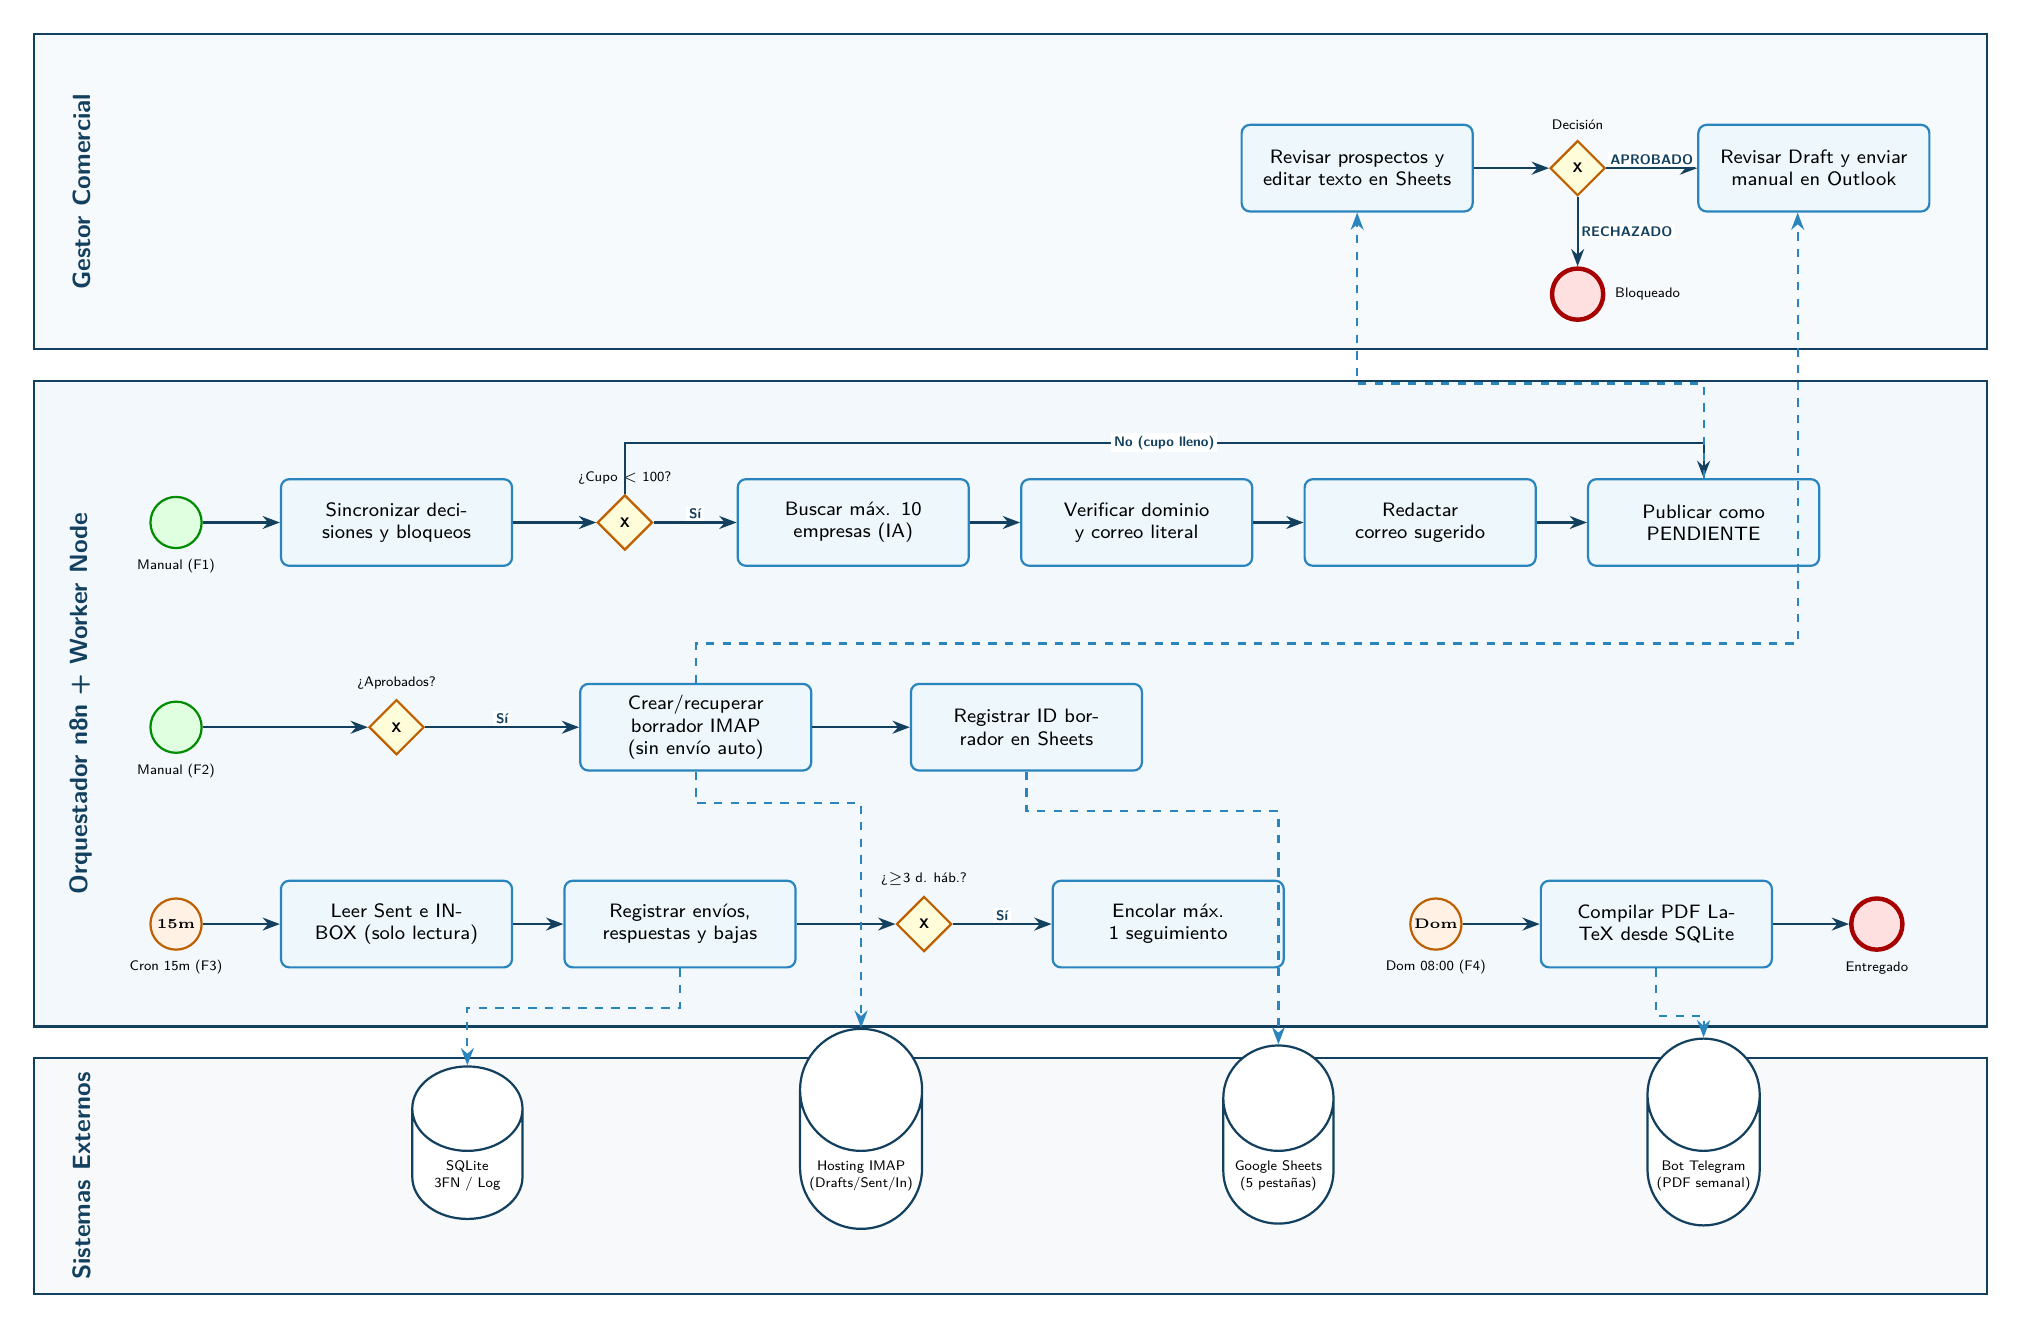
\includegraphics[width=\textwidth,height=0.72\textheight,keepaspectratio]{../informe/bpmn_prospeccion_tobe_e2.png}
\column{0.40\textwidth}
\small
\begin{itemize}
    \item \textbf{Flujo 1 (Manual):} Cupo máx. \textbf{100 pendientes}, búsqueda IA en 14 familias y verificación literal de correo en dominio.
    \item \textbf{Revisión humana:} Google Sheets (5 pestañas; solo C, H, I, J editables).
    \item \textbf{Flujo 2 (Manual):} Borradores IMAP idempotentes en \texttt{Drafts}; \textbf{cero envío automático} (\texttt{DELIVERY\_MODE=drafts}).
    \item \textbf{Flujo 3 (Cron 15m):} Monitorea \texttt{Sent}/\texttt{INBOX}, aplica bajas Ley 21.719 y prepara máx. 1 seguimiento a los \textbf{3 días hábiles}.
    \item \textbf{Flujo 4 (Dom 08:00):} PDF LaTeX semanal vía Telegram (sin IA).
\end{itemize}
\end{columns}
\end{frame}

% --- SLIDE 5: FICHAS Y ARQUITECTURA ---
\begin{frame}{4. Automatización de Fichas Técnicas y Arquitectura SIG}
\begin{columns}[T]
\column{0.54\textwidth}
\centering
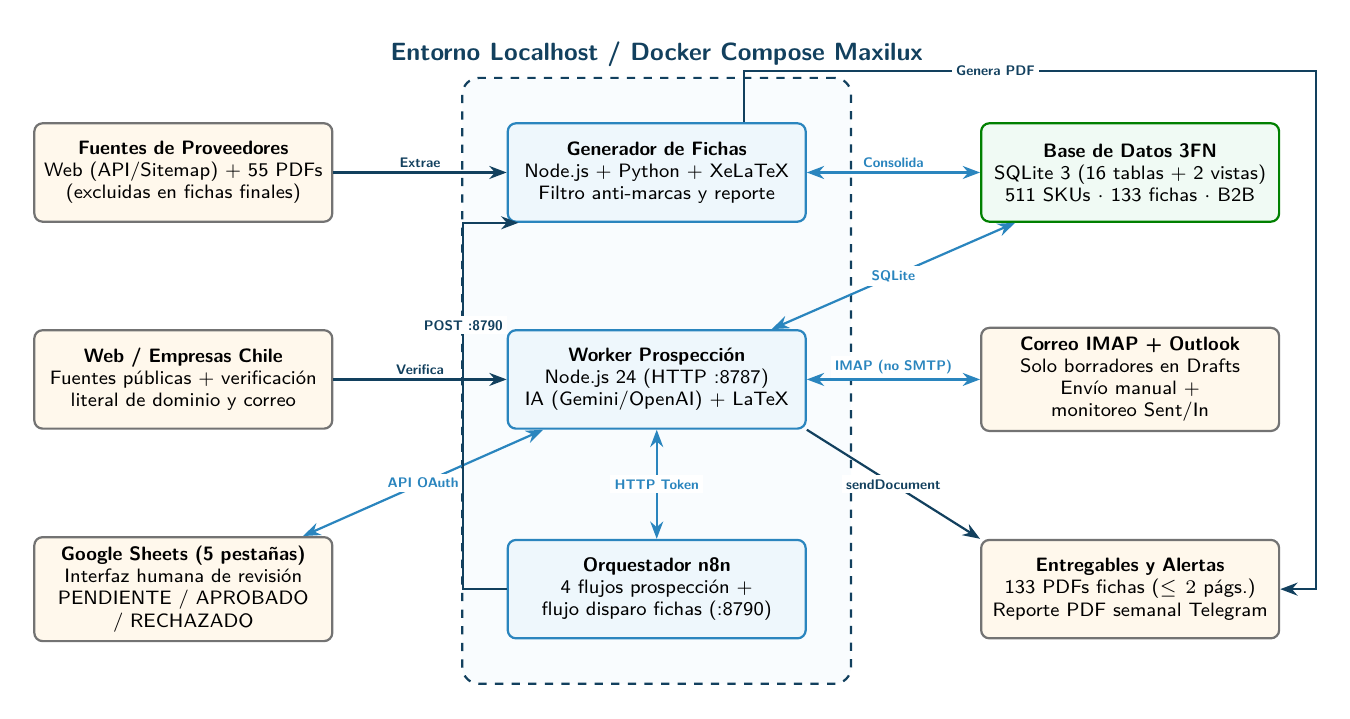
\includegraphics[width=\textwidth,height=0.72\textheight,keepaspectratio]{../informe/arquitectura_sig_maxilux.png}
\column{0.44\textwidth}
\small
\begin{block}{Generador Consolidado (\texttt{generador/})}
\begin{itemize}
    \item Disparo vía n8n (\texttt{Maxilux\_Generar\_Fichas.json}, HTTP \texttt{:8790}).
    \item Fusiona Lista (511 SKUs) + 55 PDFs + 3 webs de proveedores.
    \item \textbf{Filtro anti-marcas:} aborta si aparece un proveedor (\textbf{0 fugas}).
    \item Compila \textbf{133 PDFs XeLaTeX ($\le 2$ págs.)}: 2 \texttt{FINAL} + 131 \texttt{BORRADOR} cuando falta IP, Temp. o Cert.
\end{itemize}
\end{block}
\end{columns}
\end{frame}

% --- SLIDE 6: MODELO DE DATOS 3FN ---
\begin{frame}{5. Modelo de Datos en 3FN estricta (16 tablas + 2 vistas)}
\begin{columns}[T]
\column{0.62\textwidth}
\centering
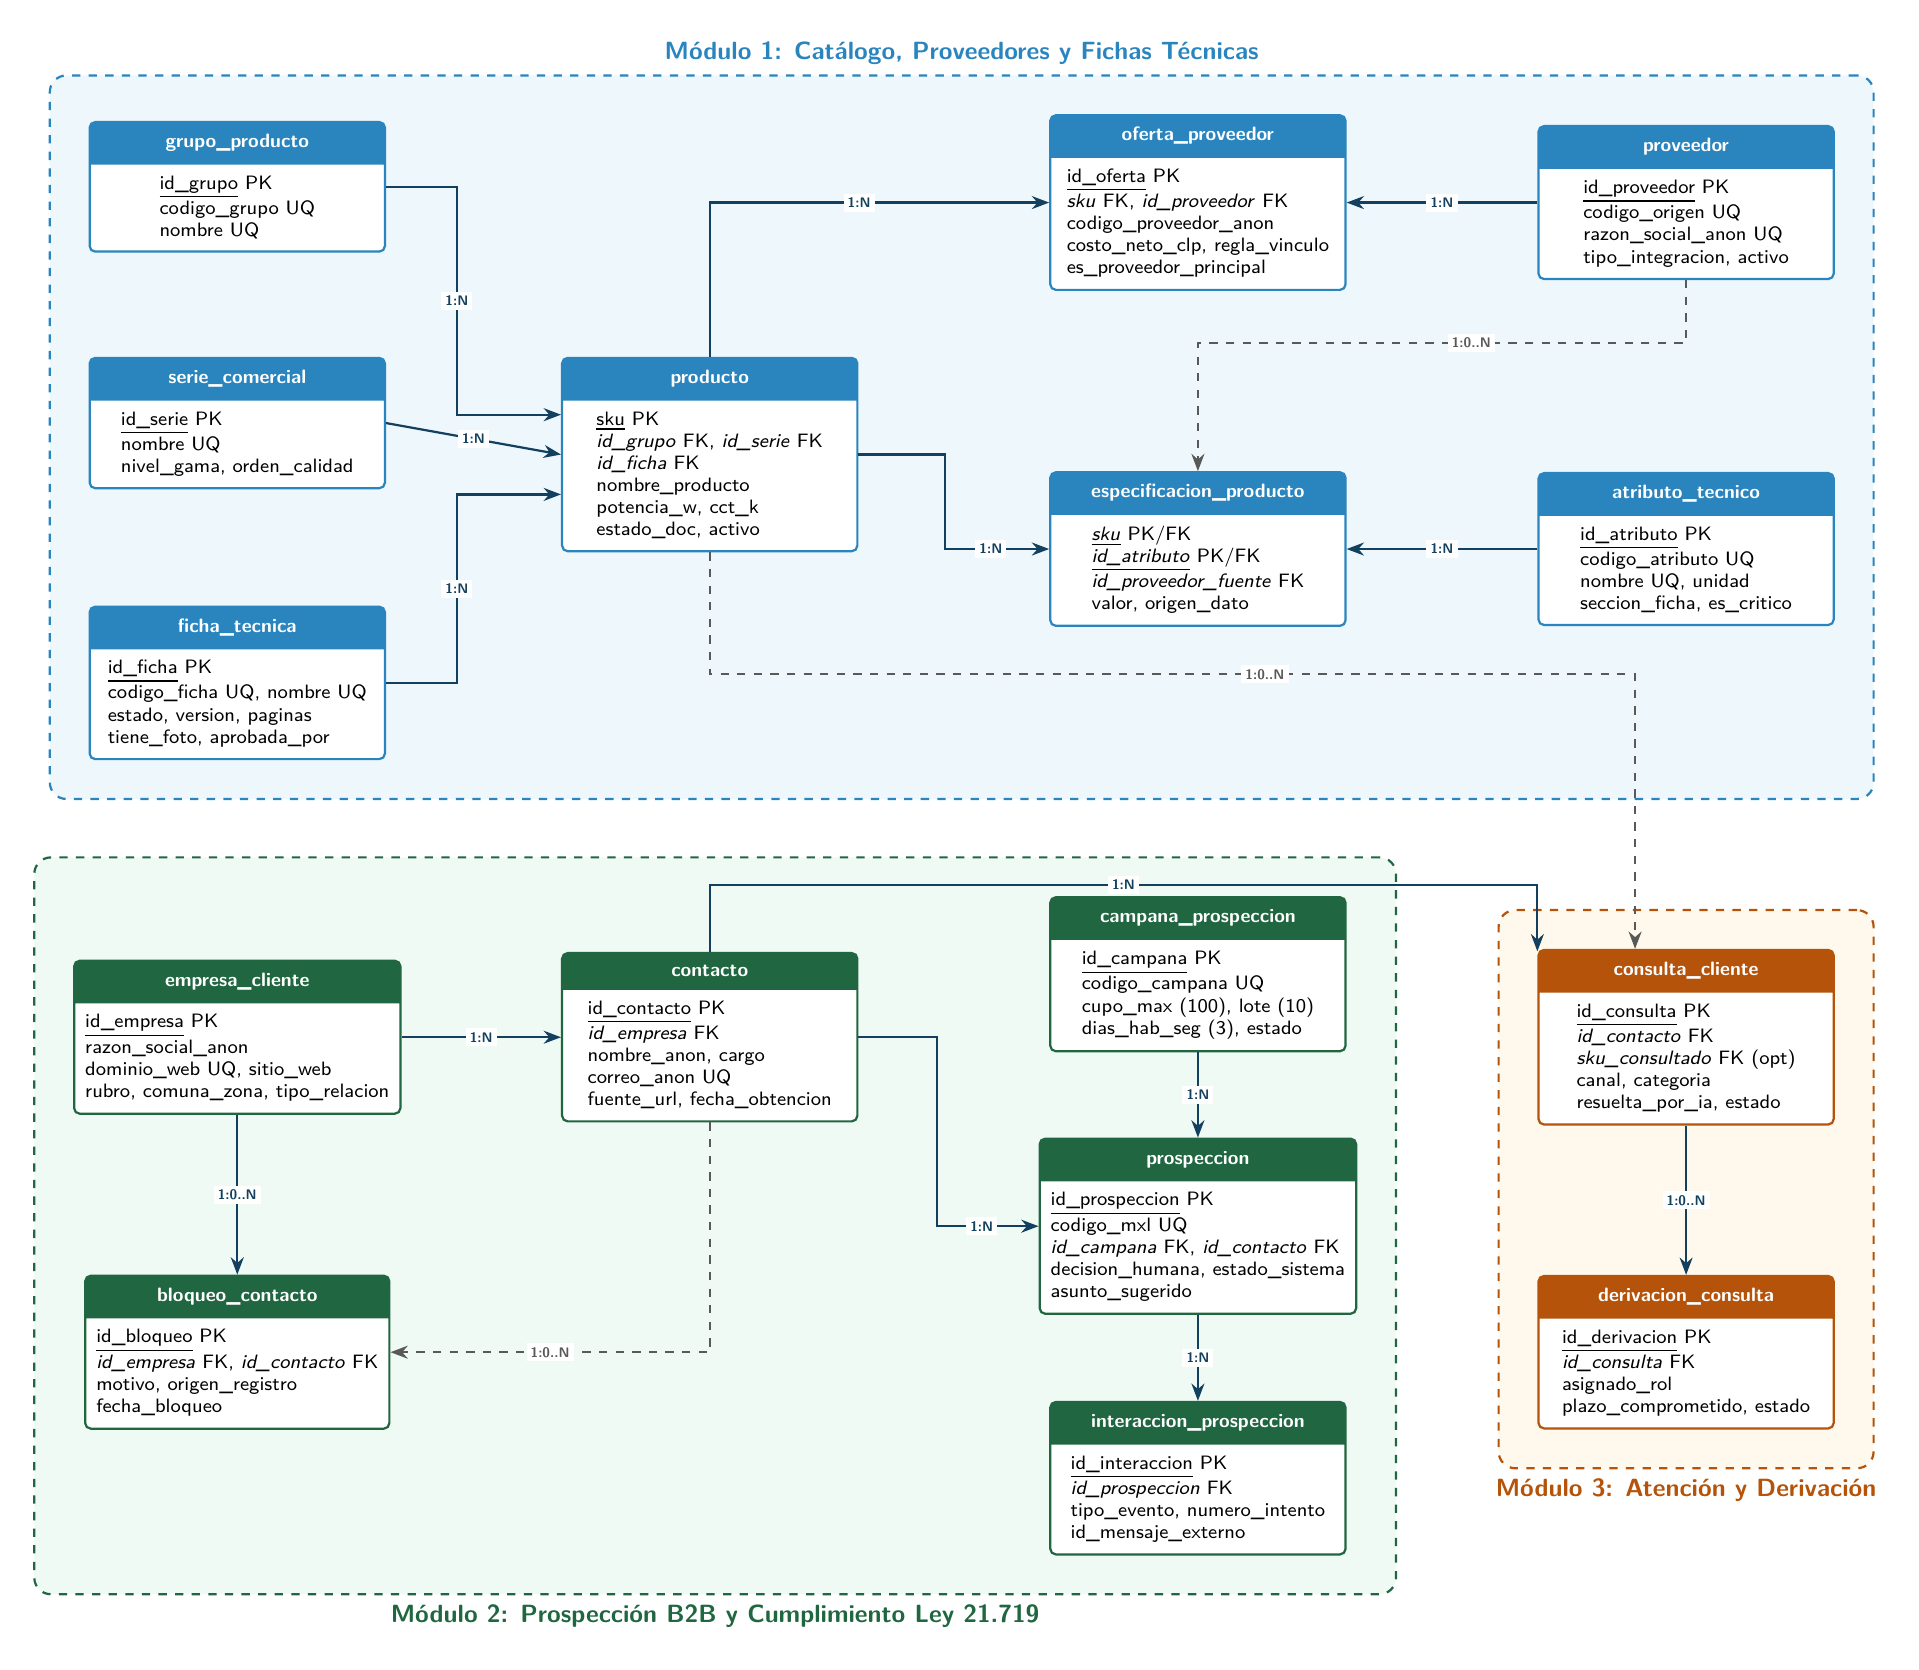
\includegraphics[width=\textwidth,height=0.75\textheight,keepaspectratio]{../informe/er_maxilux_3fn.png}
\column{0.36\textwidth}
\small
\begin{block}{Anomalías eliminadas}
\begin{itemize}
    \item \textbf{1FN:} Eliminadas columnas \texttt{Caract. 1..6} del Excel (77 cols) y blobs JSON de \texttt{leads}.
    \item \textbf{2FN:} Separación de \texttt{producto (sku)}, \texttt{oferta\_proveedor} y \texttt{especificacion\_producto}.
    \item \textbf{3FN:} Precios (\(\times 1{,}65 / 1{,}52 / 1{,}42\)) y faltantes críticos calculados en \textbf{2 vistas} sin redundancia.
\end{itemize}
\end{block}
\end{columns}
\end{frame}

% --- SLIDE 7: RESULTADOS SQL CATALOGO Y PRECIOS ---
\begin{frame}{6. Evidencia SQL (Q1--Q3): Cobertura documental y precios}
\begin{columns}[T]
\column{0.49\textwidth}
\begin{block}{Q1 y Q2: Cobertura real (511 SKUs / 133 fichas)}
\footnotesize
\begin{itemize}
    \item \textbf{323 SKUs (63,2\,\%)} con respaldo técnico vs \textbf{188 (36,8\,\%)} sin respaldo (postes, solares/baterías, calle).
    \item \textbf{Cuello de botella crítico (Q2):}
    \begin{itemize}\footnotesize
        \item \texttt{TEMP\_OPERACION}: solo \textbf{15,1\,\%} (bloquea 128 fichas).
        \item \texttt{CERTIFICACIONES}: solo \textbf{19,0\,\%} (bloquea 124 fichas).
        \item \texttt{IP}: \textbf{54,4\,\%} (bloquea 85 fichas).
    \end{itemize}
\end{itemize}
\end{block}
\column{0.48\textwidth}
\begin{block}{Q3: Corrección \texttt{MIN} vs \texttt{MAX} (32 SKUs multioferta)}
\scriptsize
\begin{tabular}{lrrr}
\toprule
\textbf{Grupo} & \textbf{SKUs} & \textbf{Prom. Mín.} & \textbf{Ahorro acum.} \\
\midrule
SOLAR Y BATERÍA & 4 & \$73.525 & \$62.500 \\
PROYECTOR & 8 & \$51.800 & \$58.100 \\
CAMPANA & 3 & \$69.633 & \$44.400 \\
PANEL LED & 17 & \$10.818 & \$32.000 \\
\midrule
\textbf{Total muestra} & \textbf{32} & --- & \textbf{\$197.000} \\
\bottomrule
\end{tabular}
\vspace{4pt}
\newline {\footnotesize Vista \texttt{v\_lista\_precios\_clientes} (costos sintéticos CLP).}
\end{block}
\end{columns}
\end{frame}

% --- SLIDE 8: RESULTADOS SQL PROSPECCION, LEY 21.719 Y ATENCION ---
\begin{frame}{7. Evidencia SQL (Q4--Q7): Prospección, Ley 21.719 y Atención}
\begin{columns}[T]
\column{0.47\textwidth}
\begin{block}{Q4--Q6: Embudo B2B y Cumplimiento}
\footnotesize
\begin{itemize}
    \item \textbf{Embudo (Q4):} 25 prospectos sintéticos en 3 campañas (7 pendientes, 4 borradores IMAP, 6 enviados, 3 respuestas reales, 5 bloqueos).
    \item \textbf{Ley 21.719 (Q5):} \textbf{0 prospecciones activas} sobre las 5 empresas bloqueadas (\texttt{SHEETS} / \texttt{IMAP\_INBOX}).
    \item \textbf{Seguimientos (Q6):} 4 envíos elegibles ($\ge 3$ días hábiles); excluye respuestas automáticas.
\end{itemize}
\end{block}
\column{0.50\textwidth}
\begin{block}{Q7: Impacto de las fichas en atención}
\scriptsize
\begin{tabular}{lrrr}
\toprule
\textbf{Estado ficha} & \textbf{Cons.} & \textbf{\% IA} & \textbf{Tiempo prom.} \\
\midrule
\texttt{COMPLETA} & 6 & \textbf{83,3\,\%} & \textbf{25,3 min} \\
\texttt{CONSULTA\_GRAL} & 2 & 50,0\,\% & 75,1 min \\
\texttt{BORRADOR} & 9 & 0,0\,\% & 470,7 min \\
\texttt{SIN\_RESPALDO} & 7 & 0,0\,\% & 1.419,0 min \\
\bottomrule
\end{tabular}
\vspace{4pt}
\newline {\footnotesize Las fichas aprobadas cierran el ciclo entre módulos.}
\end{block}
\end{columns}
\end{frame}

% --- SLIDE 9: CIERRE, LIMITACIONES Y ROLES ---
\begin{frame}{8. Cierre: logros auditables, limitaciones y equipo}
\begin{columns}[T]
\column{0.52\textwidth}
\begin{block}{Logros verificados y limitaciones honestas}
\footnotesize
\begin{itemize}
    \item \textbf{Reproducible en 1 paso:} \texttt{python db/ejecutar.py} (0 errores FK) + 66 tests unitarios n8n/Worker aprobados.
    \item \textbf{Limitación 1:} 131 de 133 fichas siguen en \texttt{BORRADOR} hasta recopilar temp./certificaciones de proveedores.
    \item \textbf{Limitación 2:} Chat de atención modelado en BD 3FN (fase futura tras aprobar fichas).
    \item \textbf{Limitación 3:} Credenciales productivas OAuth/IA/IMAP en \texttt{privado/config.env} para activación final.
\end{itemize}
\end{block}
\column{0.45\textwidth}
\begin{block}{Reparto de defensa (6:30 / 7:00 min)}
\scriptsize
\begin{tabular}{llr}
\toprule
\textbf{Integrante} & \textbf{Bloque} & \textbf{Tiempo} \\
\midrule
Juan Pablo Godoy & Contexto y problema & 1:30 \\
Vicente Soto & BPMN y flujos n8n & 1:40 \\
Joaquín Tapia & Modelo ER 3FN & 1:40 \\
Claudio Vera & SQL, Q1--Q7 y cierre & 1:40 \\
\bottomrule
\end{tabular}
\end{block}
\end{columns}
\end{frame}

\end{document}
